\documentclass[fullscreen=true, unicode, bookmarks=false]{beamer}
\usepackage[T2A]{fontenc}
\usepackage[utf8]{inputenc}
\usepackage[english, russian]{babel}
\usepackage{amsmath}
\usepackage{amsmath,amsfonts,amssymb}
\usepackage[export]{adjustbox}
\usepackage{textgreek}
\newtheorem{rustheorem}{Теорема }
\sloppy

\setbeamertemplate{navigation symbols}{}

\usetheme{Madrid}

\usecolortheme{whale}

\usefonttheme{professionalfonts} % default family is serif

\setbeamertemplate{footline}{\hspace*{.5cm}\scriptsize{\insertshorttitle
\hspace*{50pt} \hfill\hspace*{.5cm}}\vspace{5pt}} 

\setbeamercolor{bibliography entry author}{fg=black}

\title[]{ {\huge Бифуркационные особенности одной краевой задачи с нелинейным отклонением в краевом условии } }   
\author[]{{\large Л.И.~Ивановский}} 
\date{ }
\institute[]
{ ЯрГУ им. П.Г. Демидова }

\begin{document}

\begin{frame}
\titlepage
\end{frame} 

\begin{frame}
\frametitle{ Краевая задача с отклонением в краевом условии }
 
\begin{equation}
	\dot u = u'' + \gamma u,	
\end{equation}

\begin{equation}
	u'(0, t) \, = 0, \qquad u'(1, t) \, = \alpha\,u(x_0, t) + \beta u^3(x_0, t),
\end{equation}

\bigskip

$$ t \geqslant 0, \quad x \in [0,1]. $$


$$ \alpha, \beta, \gamma \in \mathbb{R}, \quad x_0 \in [0, 1). $$

\end{frame}

\begin{frame}
\frametitle{ Линеаризованная краевая задача }
 
\begin{equation}
	\dot u = u'' + \gamma u,	
\end{equation}

\begin{equation}	
	u'(0, t) \, = 0, \qquad u'(1, t) \, = \alpha\,u(x_0, t).
\end{equation}

\end{frame}

\begin{frame}
\frametitle{ Задача на собственные значения }
 
$$ u(x, t) = e^{\lambda t} \, v(x). $$

\bigskip
 
\begin{equation}
	v'' + (\gamma - \lambda)v = 0,	
\end{equation}

\begin{equation}	
	v'(0) \, = 0, \qquad v'(1) \, = \alpha\,v(x_0).
\end{equation}

\bigskip

$$ \mu = \sqrt{-\gamma + \lambda}, $$

$$ v(x) = c \ch  \mu x, \quad c \in \mathbb{R}. $$

\end{frame}

\begin{frame}
\frametitle{ Потеря устойчивости нулевого состояния равновесия }
 
\begin{equation}
	\mu \, \sh \mu \, = \, \alpha \ch \mu x_0,
\end{equation}

\medskip

\begin{itemize}

\item { $ \lambda = 0: \; \mu = \sqrt{-\gamma}, $ 
}

$$ \alpha_u = \frac{ \sqrt{-\gamma} \, \sh \sqrt{-\gamma} }{ \ch \sqrt{-\gamma} x_0 }. $$

\item { $ \lambda = \pm i \omega: \; \mu = \sqrt{-\gamma + i \omega}, $ 
}

$$ \alpha_c = \frac{ \sqrt{-\gamma + i \omega} \, \sh \sqrt{-\gamma + i \omega} }{ \ch \sqrt{-\gamma + i \omega} x_0 }. $$

\end{itemize}	

\end{frame}

\begin{frame}
\frametitle{ Построение зависимости $ \alpha_c(\gamma) $ }
 
\begin{itemize}

\item { $ \gamma = 0, \, x_0 = 0: $ 
\begin{equation}
 \begin{cases}
   \tg \, y + \th \, y = 0, 
   \\
   \alpha_c = y(\sh y \cos y - \ch y \sin y),
 \end{cases}
\end{equation}
$$ y = \sqrt{ \frac{\omega}{2} }. $$
}

\item { $ \gamma = 0, \, x_0 \neq 0: $ 
\begin{equation}
 \begin{cases}
   \dfrac{\sh y \cos y + \ch y \sin y}{\sh y \cos y - \ch y \sin y} - \tg y x_0 \th y x_0 = 0, 
   \vspace{0.1cm}
   \\ 
   \alpha_c = \dfrac{y \sh y \cos y - y \ch y \sin y}{\ch y x_0 \cos y x_0}.
 \end{cases}
\end{equation}
}

\item { $ \gamma \neq 0, \, x_0 \neq 0. $ 
}

\end{itemize}	

\end{frame}

\begin{frame}
\frametitle{ Численные результаты: $ \alpha_c(x_0) $ при $ \gamma = 0 $ }

\begin{figure} 
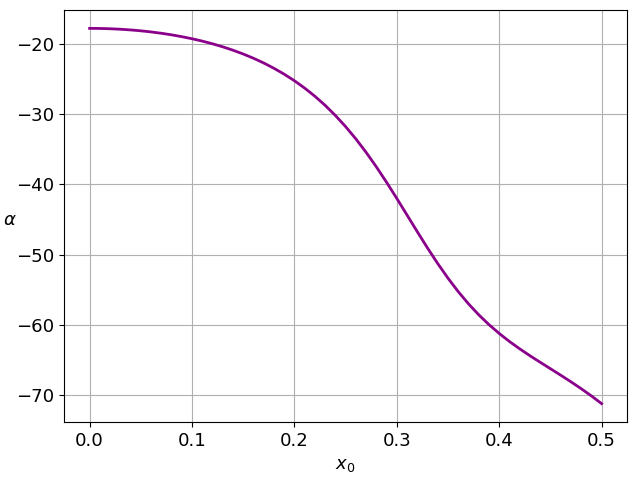
\includegraphics[scale=0.65]{origins.png}  
\end{figure}

\end{frame}

\begin{frame}
\frametitle{ Численные результаты: $ \omega(\gamma) $ }

\begin{figure} 
\begin{minipage}[h]{0.49\linewidth}
\begin{center}
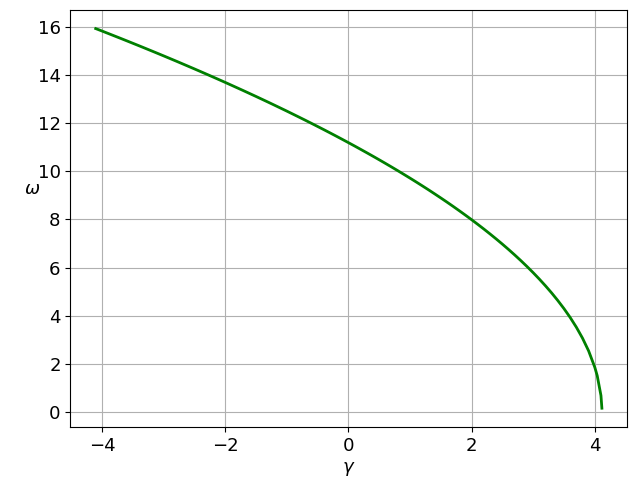
\includegraphics[scale=0.35]{omegas_x0=0,0.png} \\ {\scriptsize a) $ x_0 = 0.0 $}
\end{center}
\end{minipage} 
\hfill
\begin{minipage}[h]{0.49\linewidth}
\begin{center}
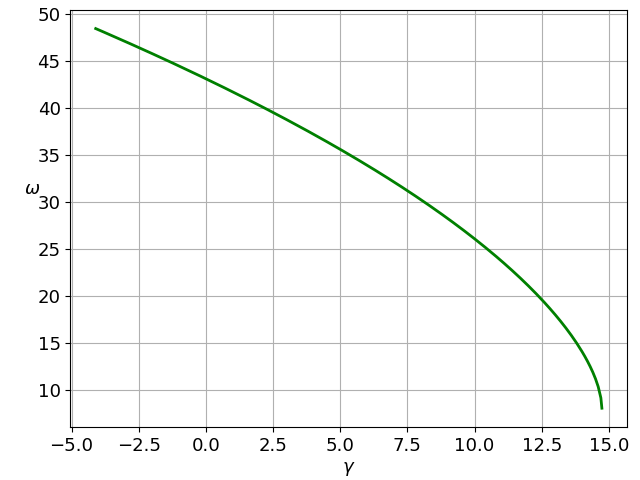
\includegraphics[scale=0.35]{omegas_x0=0,5.png}  \\ {\scriptsize b) $ x_0 = 0.5 $}
\end{center}
\end{minipage} 
\end{figure}

\end{frame}

\begin{frame}
\frametitle{ Моделирование линейной краевой задачи }

\begin{equation}\label{numeric_problem} 
	\dot{u}_j =  n^2(u_{j+1} - 2u_j + u_{j-1}) + \gamma u_j, \quad j = \overline{1, n}, 
\end{equation}

\vfill

$$ u_0 = u_1, $$
$$ u_{n+1} = u_n + \frac{\alpha}{n}\:u_k, \quad k \in [1,n]. $$

\end{frame}

\begin{frame}
\frametitle{ Схематическая визуализация критической зависимости }

\begin{figure} 
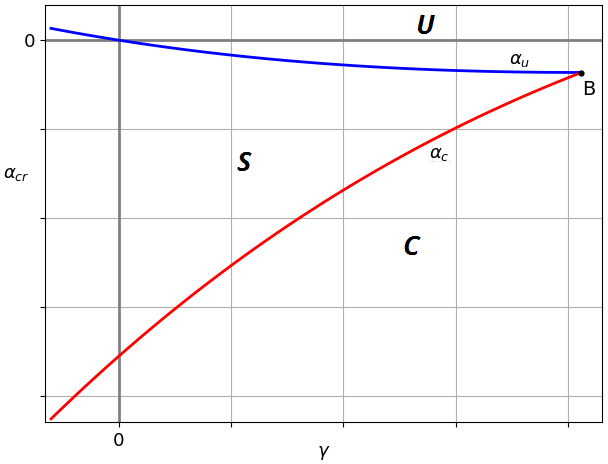
\includegraphics[scale=0.55]{scheme.png}  
\end{figure}

$$ B=(\gamma_*, \alpha_*) $$

\end{frame}

\begin{frame}
\frametitle{ Численные результаты: $ \alpha_{cr}(\gamma) $ }

\begin{figure} 
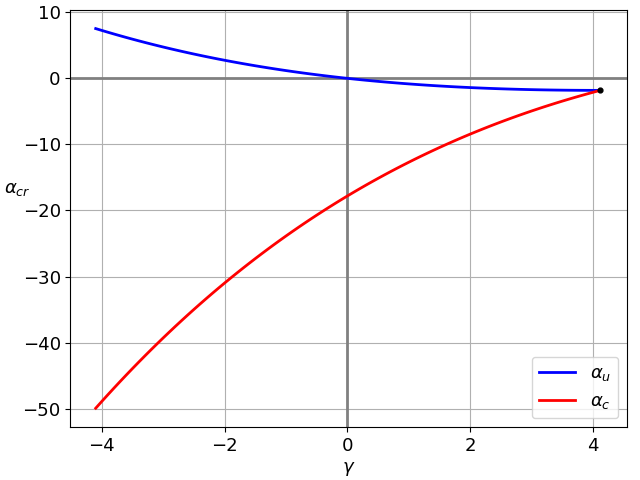
\includegraphics[scale=0.55]{alphas_0.png}  
\end{figure}

$$ x_0 = 0: \quad \gamma_* \approx 4.115 $$

\end{frame}

\begin{frame}
\frametitle{ Численные результаты: $ \alpha_{cr}(\gamma) $ }

\begin{figure} 
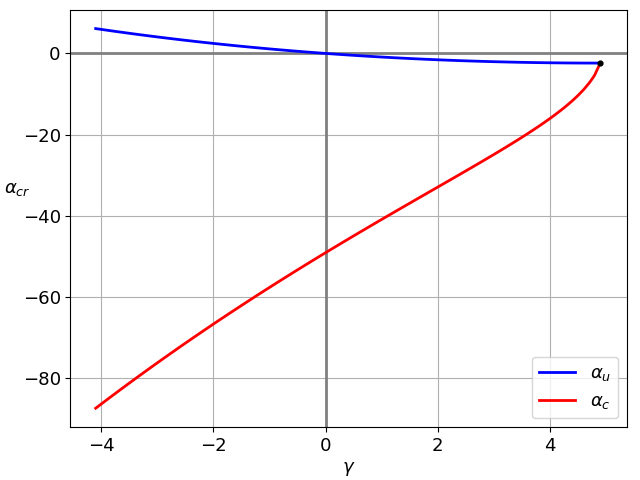
\includegraphics[scale=0.55]{alphas_13.png}  
\end{figure}

$$ x_0 = 0.33: \quad \gamma_* \approx 4.895 $$

\end{frame}

\begin{frame}
\frametitle{ Численные результаты: $ \alpha_{cr}(\gamma) $ }

\begin{figure} 
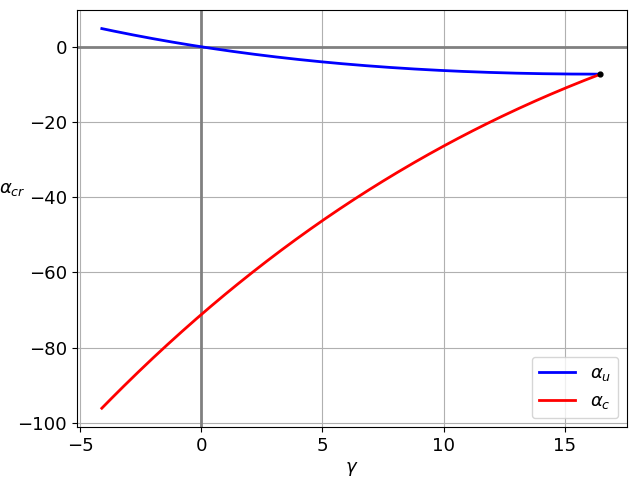
\includegraphics[scale=0.55]{alphas_12.png}  
\end{figure}

$$ x_0 = 0.5: \quad \gamma_* \approx 16.4 $$

\end{frame}

\begin{frame}
\frametitle{ Численные результаты: $ \alpha_{cr}(\gamma) $ }

\begin{figure} 
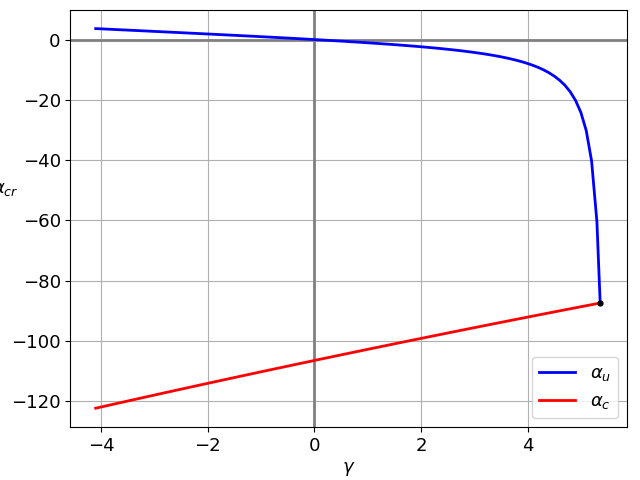
\includegraphics[scale=0.55]{alphas_23.png}  
\end{figure}

$$ x_0 = 0.67: \quad \gamma_* \approx 5.361 $$

\end{frame}

\begin{frame}
\frametitle{ Локальный анализ краевой задачи }

\begin{equation}
	u = \sqrt{\varepsilon}u_0 + \varepsilon u_1 + \varepsilon^{\frac{3}{2}} u_2 + O(\varepsilon^2),
\end{equation}

\bigskip

$$ \varepsilon = | \alpha - \alpha_{cr} |, $$

$$ \varepsilon \ll 1, \quad s = \varepsilon t. $$

\end{frame}

\begin{frame}
\frametitle{ Случай дивергентной потери устойчивости }

\begin{itemize}
\item { $ \lambda = 0: \quad \varepsilon=\alpha-\alpha_u, $
}
\end{itemize}

\medskip

\begin{equation}
	u_0 = u_0'' + \gamma u_0,
\end{equation}
\begin{equation}
	u_0'(0, t) \, = 0, \qquad u_0'(1, t) \, = \alpha_u u_0(x_0, t),
\end{equation}

$$ u_0 = \rho(s) \ch \sqrt{-\gamma} x. $$

\medskip

\begin{equation}
	\dot u_2 + \frac{\partial u_0}{\partial s} = u_2'' + \gamma u_2 - u_0^3,
\end{equation}
\begin{equation}
	u_2'(0, t) \, = 0, \qquad u_2'(1, t) \, = \alpha_u u_2(x_0, t) + u_0(x_0, t) + \beta u_0^3(x_0, t),
\end{equation}

\end{frame}

\begin{frame}
\frametitle{ Случай дивергентной потери устойчивости }

$$ u_2 = e^{\lambda t}v_2(x), \quad \lambda = 0, $$

\medskip

\begin{equation}
	v_2'' + \gamma v_2 - \rho' \ch \sqrt{-\gamma} x = 0,
\end{equation}
\begin{equation}
	v_2'(0) \, = 0, \quad v_2'(1) \, = \alpha_u v_2(x_0) + \rho \ch \sqrt{-\gamma} x_0 + \beta \rho^3\ch^3 \sqrt{-\gamma} x_0.
\end{equation}

\medskip

$$ v_2(x) = c\,\ch \sqrt{-\gamma} x + \frac{\rho'}{2\sqrt{-\gamma}}\sh\sqrt{-\gamma}x + \frac{\rho'x}{2} \ch\sqrt{-\gamma}x. $$
$$ c \in \mathbb{R}. $$

\end{frame}

\begin{frame}
\frametitle{ Случай дивергентной потери устойчивости }

\begin{equation}
	\rho' = \phi_0 \rho + d_0 \rho^3,
\end{equation}

\bigskip

$$ \phi_0 = Q \ch \sqrt{-\gamma} x_0, $$
$$ d_0 = \beta Q \ch^3 \sqrt{-\gamma} x_0, $$

$$ Q = \frac{2\sqrt{-\gamma}}{\sqrt{-\gamma}\ch\sqrt{-\gamma} + \sh\sqrt{-\gamma} - \alpha_u x_0 \sqrt{-\gamma} x_0}. $$

\end{frame}

\begin{frame}
\frametitle{ Численные результаты: $ \phi_0(\gamma) $ и $ d_0(\gamma) $ }

\begin{figure} 
\begin{minipage}[h]{0.49\linewidth}
\begin{center}
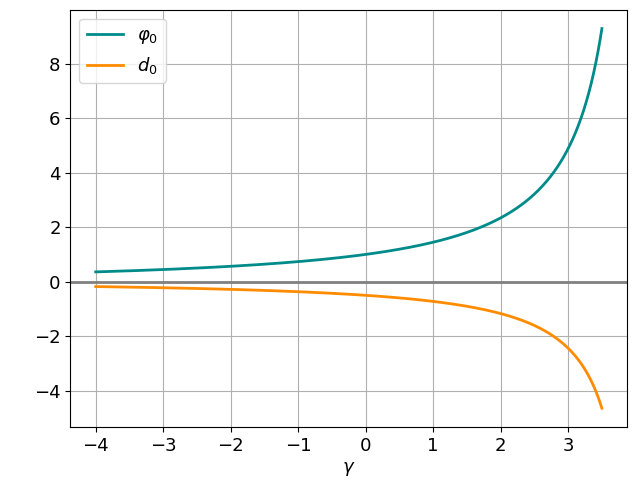
\includegraphics[scale=0.38]{divergent_phi0d0_x0=0,0,beta=-0,5.png} \\ {\scriptsize a) $ \beta = -0.5 $}
\end{center}
\end{minipage} 
\hfill
\begin{minipage}[h]{0.49\linewidth}
\begin{center}
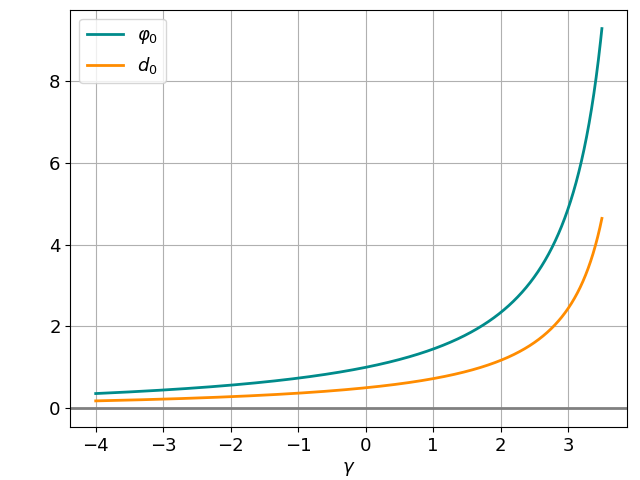
\includegraphics[scale=0.38]{divergent_phi0d0_x0=0,0,beta=0,5.png}  \\ {\scriptsize b) $ \beta = 0.5 $}
\end{center}
\end{minipage} 
\end{figure}

$$ x_0 = 0.0 $$

\end{frame}

\begin{frame}
\frametitle{ Численные результаты: $ \phi_0(\gamma) $ и $ d_0(\gamma) $ }

\begin{figure} 
\begin{minipage}[h]{0.49\linewidth}
\begin{center}
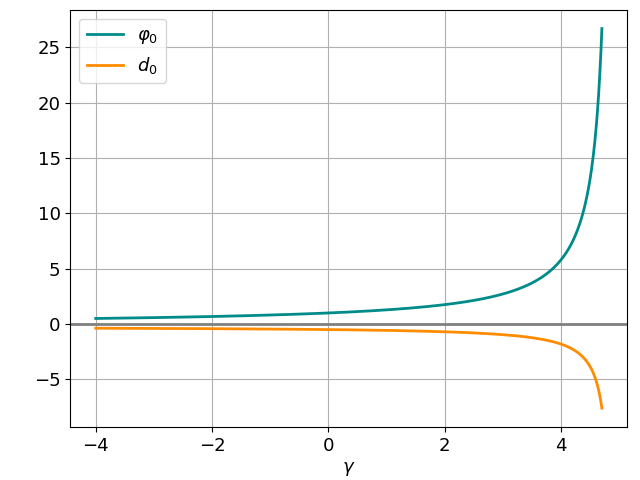
\includegraphics[scale=0.38]{divergent_phi0d0_x0=0,33,beta=-0,5.png} \\ {\scriptsize a) $ \beta = -0.5 $}
\end{center}
\end{minipage} 
\hfill
\begin{minipage}[h]{0.49\linewidth}
\begin{center}
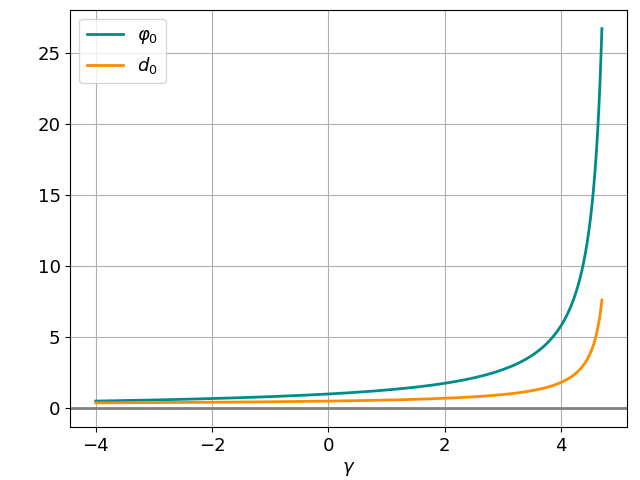
\includegraphics[scale=0.38]{divergent_phi0d0_x0=0,33,beta=0,5.png}  \\ {\scriptsize b) $ \beta = 0.5 $}
\end{center}
\end{minipage} 
\end{figure}

$$ x_0 = 0.33 $$

\end{frame}

\begin{frame}
\frametitle{ Численные результаты: $ \phi_0(\gamma) $ и $ d_0(\gamma) $ }

\begin{figure} 
\begin{minipage}[h]{0.49\linewidth}
\begin{center}
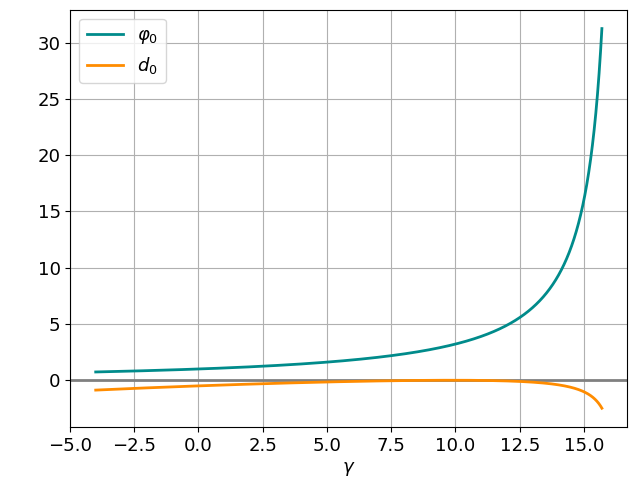
\includegraphics[scale=0.38]{divergent_phi0d0_x0=0,5,beta=-0,5.png} \\ {\scriptsize a) $ \beta = -0.5 $}
\end{center}
\end{minipage} 
\hfill
\begin{minipage}[h]{0.49\linewidth}
\begin{center}
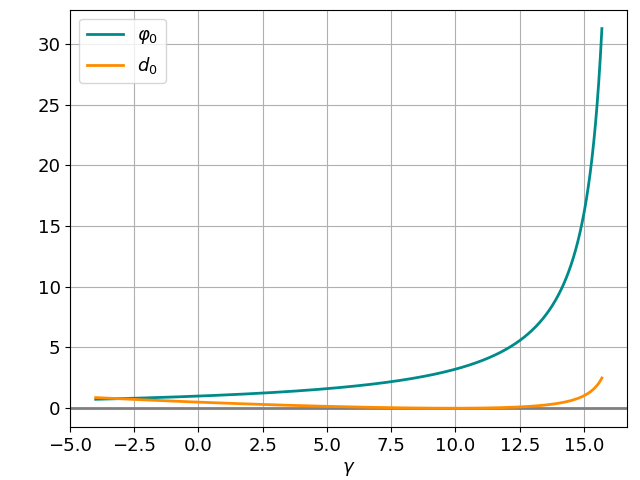
\includegraphics[scale=0.38]{divergent_phi0d0_x0=0,5,beta=0,5.png}  \\ {\scriptsize b) $ \beta = 0.5 $}
\end{center}
\end{minipage} 
\end{figure}

$$ x_0 = 0.5 $$

\end{frame}

\begin{frame}
\frametitle{ Численные результаты: $ \phi_0(\gamma) $ и $ d_0(\gamma) $ }

\begin{figure} 
\begin{minipage}[h]{0.49\linewidth}
\begin{center}
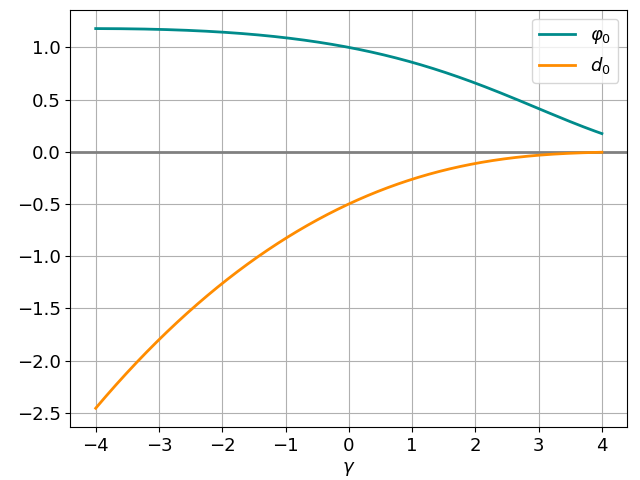
\includegraphics[scale=0.38]{divergent_phi0d0_x0=0,67,beta=-0,5.png} \\ {\scriptsize a) $ \beta = -0.5 $}
\end{center}
\end{minipage} 
\hfill
\begin{minipage}[h]{0.49\linewidth}
\begin{center}
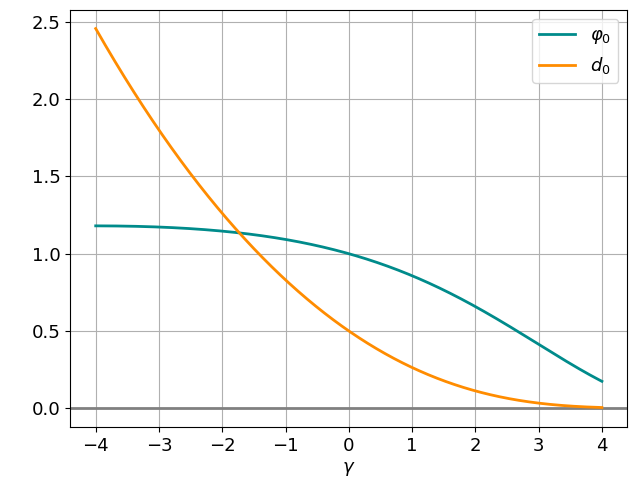
\includegraphics[scale=0.38]{divergent_phi0d0_x0=0,67,beta=0,5.png}  \\ {\scriptsize b) $ \beta = 0.5 $}
\end{center}
\end{minipage} 
\end{figure}

$$ x_0 = 0.67 $$

\end{frame}

\begin{frame}
\frametitle{ Случай колебательной потери устойчивости }

\begin{itemize}
\item { $ \lambda = \pm i \omega: \quad \varepsilon=\alpha_c-\alpha, $
}
\end{itemize}

\medskip

\begin{equation}
	u_0 = u_0'' + \gamma u_0,
\end{equation}
\begin{equation}
	u_0'(0, t) \, = 0, \qquad u_0'(1, t) \, = \alpha_c u_0(x_0, t),
\end{equation}

$$ u_0 = z(s) e^{i \omega t} \ch \mu x + \overline{z(s)} e^{-i \omega t} \overline{\ch \mu x}. $$

\medskip

\begin{equation}
	\dot u_2 + \frac{\partial u_0}{\partial s} = u_2'' + \gamma u_2,
\end{equation}
\begin{equation}
	u_2'(0, t) \, = 0, \qquad u_2'(1, t) \, = \alpha_c u_2(x_0, t) - u_0(x_0, t) + \beta u_0^3(x_0, t).
\end{equation}

\end{frame}

\begin{frame}
\frametitle{ Случай колебательной потери устойчивости }

$$ u_2 = e^{i \omega t} v_2(x), $$

\bigskip

\begin{equation}
	v_2'' + (\gamma - i \omega) v_2 - z' w(x) = 0,
\end{equation}
\begin{equation}
	v_2'(0) \, = 0, \qquad v_2'(1) \, = \alpha_u v_2(x_0) - z w(x_0) + 3\beta z|z|^2 w|w|^2.
\end{equation}

$$ w(x) = \ch \sqrt{-\gamma + i \omega} \, x. $$

\end{frame}

\begin{frame}
\frametitle{ Случай колебательной потери устойчивости }

\begin{equation}
	z' = \phi_0 z + d_0 z |z|^2,
\end{equation}

\bigskip

$$ \phi_0 = -2 \operatorname{Re} (Q\ch \mu x_0), $$

$$ d_0 = 1.5 \beta \operatorname{Re} (Q ( \ch(\mu + 2\,\mbox{Re}\mu)x_0 + \ch(\mu + 2i\,\mbox{Im}\mu)x_0 + 2\ch\overline{\mu}x_0 )), $$

\bigskip

$$ \mu = \sqrt{-\gamma + i \omega}, $$

$$ Q = \frac{\mu}{\mu \ch \mu + \sh \mu - \alpha_c x_0 \sh \mu x_0}. $$

\end{frame}

\begin{frame}
\frametitle{ Численные результаты: $ \phi_0(\gamma) $ и $ d_0(\gamma) $ }

\begin{figure} 
\begin{minipage}[h]{0.49\linewidth}
\begin{center}
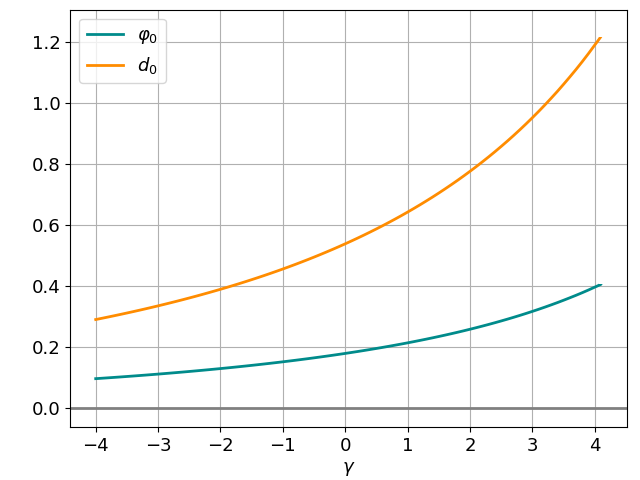
\includegraphics[scale=0.35]{oscillating_phi0d0_x0=0,0,beta=-1,0.png} \\ {\scriptsize a) $ \beta = -1.0 $}
\end{center}
\end{minipage} 
\hfill
\begin{minipage}[h]{0.49\linewidth}
\begin{center}
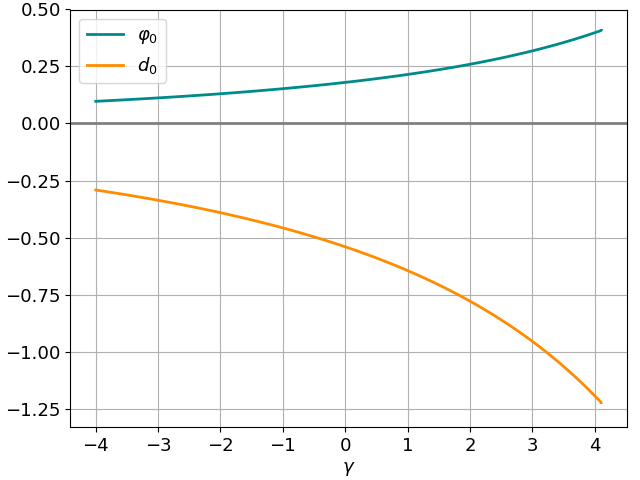
\includegraphics[scale=0.35]{oscillating_phi0d0_x0=0,0_beta=1,0.png}  \\ {\scriptsize b) $ \beta = 1.0 $}
\end{center}
\end{minipage} 
\end{figure}

$$ x_0 = 0.0 $$

\end{frame}

\begin{frame}
\frametitle{ Численные результаты: $ \phi_0(\gamma) $ и $ d_0(\gamma) $ }

\begin{figure} 
\begin{minipage}[h]{0.49\linewidth}
\begin{center}
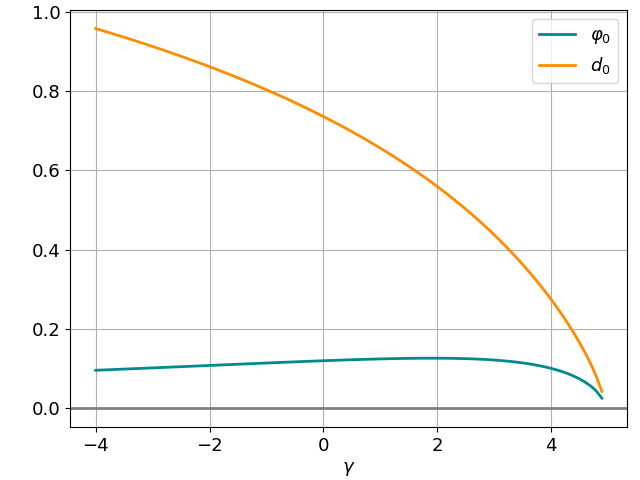
\includegraphics[scale=0.35]{oscillating_phi0d0_x0=0,33,beta=-1,0.png} \\ {\scriptsize a) $ \beta = -1.0 $}
\end{center}
\end{minipage} 
\hfill
\begin{minipage}[h]{0.49\linewidth}
\begin{center}
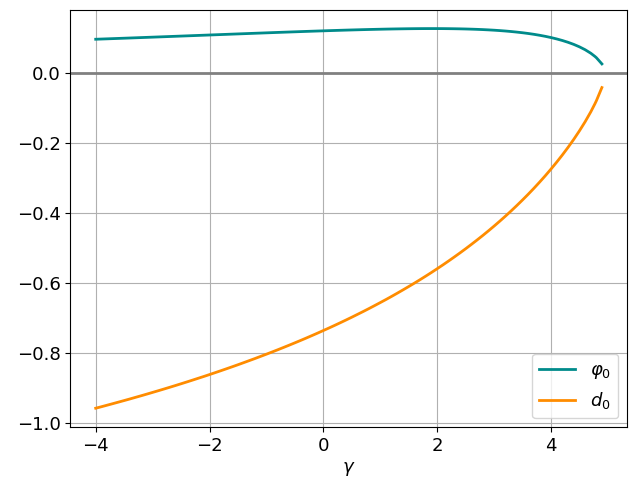
\includegraphics[scale=0.35]{oscillating_phi0d0_x0=0,33,beta=1,0.png}  \\ {\scriptsize b) $ \beta = 1.0 $}
\end{center}
\end{minipage} 
\end{figure}

$$ x_0 = 0.33 $$

\end{frame}

\begin{frame}
\titlepage
\end{frame} 

\end{document}